\chapter{Grundlagen}
\label{chapter:grundlagen}

\section{Verwandte Werke}
Bussman et al. erklärt in \cite{Bussmann2006} Impulse, die durch neue Technologien ausgelöst werden können. Dabei wird auch auf die damit verbundene mögliche Modernisierung von Anwendungen im Finanzdienstleistungsbereich eingegangen. Diese wird durch einen Ansteig der Anforderungen in produktionsnahen, operativen Systemen \cite{Bussmann2006, Brockhoff2006} bedingt. Hierfür nennt er zwei spezifische Ansätze. Danach wird die Rolle der IT-Architektur in Verbindung mit der IT-Strategie beschrieben und eine hohe Flexibilität und Schnelligkeit gefordert. Für eine kontinuierliche Anpassung der IT-Architektur, die für den Erfolg wichtig ist \cite{Bussmann2006}, werden die damit verbundenen Schwierigkeiten genannt. Anschließend werden in einem Ausblick große Auswirkungen der IT auf die etablierten Geschäftsmodelle erwartet. Die Ergebnisse von Bussman et al. sind sehr relevant, da die Auswirkungen von neuen Technologien auf das Geschäftsmodell vorausgesehen werden und Bedingungen für den Umgang mit Technologientrends gestellt werden.
\medskip
\\
Brockhoff beschreibt in \cite{Brockhoff2006} die Hintergründe und Probleme der IT-Architektur in Banken und stellt Anforderungen an ihre IT-Architektur. Dabei fordert er die eine \ac{SOA}, um die mangelnde Flexibilität und Skalierbarkeit der alten Architektur zu beseitigen. Die Schilderungen von Brockhoff geben die Probleme in der unflexiblen IT-Architektur aus Sicht des Finanzwesens wieder.
\medskip
\\
Gupta und Simonds beschreiben in \cite{Gupta:2017} Goldman Sachs' Weg der digitalen Transformation hin zu einem Technologieunternehmen und Plattform. 
Die Studie von Gupta und Simonds stellt viele Ansätze vor, mit denen Goldman Sachs erfolgreich neue Geschäftsmodelle entwickelt hat und alte Modelle Strukturen abgeschafft hat. Diese Ansätze könnten als Positivbeispiel für das deutsche Finanzwesen dienen.
\medskip
\\
Disterer beschreibt in \cite{mci/Disterer2011} eine problematische Inbetriebnahme von Anwendungen durch die mangelnde Beachtung von nichtfunktionalen Anforderungen bei der Entwicklung. Hierzu stellt er als Lösungsansatz eine Erweiterung eines ITILv3 Prozesses mit Quality Gates, die als Synchronisationspunkt für die Koordination zwischen Entwicklung und Betrieb dienen. Der Ansatz von Disterer gibt eine Referenz für eine bessere Koordination zwischen Entwicklung und Betrieb.
\medskip
\\
Alt et al. erklärt bezogen auf das IT-Management in \cite{Alt2017} das Potenzial von DevOps zur Steigerung der Innovationsfähigkeit. Dieser ergibt sich aus Kontinuitätskonzepten und ihrer Verbindung mit einer inoovationsfokussierten IT-Strategie. Hierfür erklärt er die DevOps Prinzipien, worin er für das Kontinuitätsprinzip auf den Ansatz \emph{Continuous Delivery} eingeht. 
\medskip
\\
Pathania zeigt in \cite{Pathania2017} wie Jenkins mit Kubernetes, Docker und Public-Cloud skaliert werden kann. Dabei konfiguriert er Jenkins für die Nutzung innerhalb einer Public-Cloud und Kubernetes. Er veranschaulicht einen Ansatz, um den Jenkins Master über Replikas zu skalieren. Zudem beschreibt er die Skalierung von Jenkins Agenten für die Verteilung der Builds. Für die Agenten werden Images erzeugt, woraus Jenkins mithilfe eines Docker Plugins einen Container für den Build generiert. Für die Agenten erstellt er ein Image aus Ubuntu und installiert die Build-Tools, wie in jedem anderen Ubuntu System.
Dadurch erzeugt er die Images über einen Container, welches vorher konfiguriert wurde. Insbesondere beschreibt Pathania ausführlich die einzelnen Schritte, die für die Orchestrierung der ganzen Anwendung mit Kubernetes erforderlich sind.

\section{Stand der Technik}
Software hat eine Schlüsselrolle für digitale Innovation in allen Bereichen \cite{Alt2017}, die wichtiger denn je geworden ist. Die IT ist ständigen Veränderungen ausgesetzt. Technologietrends erzeugen immer wieder neue Impulse und Betriebe mit properietären Infrastrukturen müssen sich neu ausrichten \cite{Bussmann2006}.

So entstehen gegenüber etablierten Unternehmen, Technologieunternehmen mit effizienten Geschäftsmodellen. Sie integrieren mit unterstützenden Anwendungen IT und Geschäftsmodell \cite{Bussmann2006}. Im Finanzwesen sind es die sogenannten FinTechs \ref{Disruption:FinTechs}
\medskip
\\
Zuletzt hat sich die IT vor allem durch einige Schlüsseltechnologien verändert. Für die IT-Architektur hat Cloud-Computing zusammen mit Cloud-Plattformen einen entscheidenden Impuls gegeben. Sie haben IT-Ressourcen abstrahiert. Diese können mit Befehlen aufgerufen werden und sind in kurzer Zeit bereitgestellt. Anwendungen können in kürzester Zeit und in großem Umfang skaliert werden. Software wird dadurch immer mehr als Dienstleistung bereitgestellt und findet sich immer weniger in den Festplatten von lokalen Systemen. Kurze Entwicklungszyklen durch neue und agile Methoden sorgen für eine kontinuierliche Weiterentwicklung der Anwendungen. Software wird dadurch in immer kürzeren Abständen integriert und ausgeliefert. Hierzu entstand der Bedarf einer erhöhten Zusammenarbeit zwischen Betrieb und Entwicklung, woraus der Trendbegriff DevOps entstand. Die Kontinuität wird immer relevanter, sodass Methoden wie \ac{CI} und \ac{CD} zum Standard und miteinander vereint werden. Gleichzeitig herrscht ein kontinuierlicher Anstieg der Anforderungen an die IT-Architektur \cite{Bussmann2006}, die in unflexiblen Architekturen in einem Engpass gemündet ist \cite{Brockhoff2006, Bussmann2006}. Diese Engpässe könnten aufgrund neuer Technologien und Architekturen, wie zum Beispiel Kubernetes, Docker und Microservices gelöst werden. Grundlage hierfür bieten unter anderem gemeinsame Plattformen, wie zum Beispiel eine Cloud.

\paragraph{DevOps}
DevOps ist eine Bezeichnung, die durch die Zusammensetzung der Wörter \enquote{Development} und \enquote{Operations} erzeugt wurde und entstand aus Problemen bei der Inbetriebnahme von Software \cite{mci/Disterer2011}. Aus einer schnellen, flexiblen und nutzerzentrierten Umsetzung von funktionalen Anforderungen resultieren Benutzerakzeptanz und Kundenzufriedenheit \cite{mci/Disterer2011, Alt2017}. Daher ist es ein Ziel von DevOps die Zusammenarbeit zwischen Entwicklung und Betrieb zu verbessern. Die Automatisierung von Routineaufgaben und Wandel in der Zusammenarbeitskultur hat darin eine zentrale Bedeutung \cite{Alt2017}. 

In der Praxis werden Entwicklung und Betrieb durch die Delivery Pipeline verbunden.
Hierbei werden vor allem zwei Verfahren vereint und automatisiert, Continuous Integration und Continuous Delivery. Zusammen bilden sie einen kontinuierlichen Lebenszyklus der Entwicklung von der Idee bis hin zur Inbetriebnahme.
\medskip
\\
Für die DevOps Prinzipien gibt es keine festgelegten Beschreibungen, sodass Unternehmen sie nach ihrem eigenen Bedarf anpassen und individualisieren \cite{Alt2017}. DevOps ist ein Zusammenschluss aus mehreren Prinzipien für eine bessere Zusammenarbeit.

Es gibt jedoch Prinzipien, die vor allem eine Kulturänderung in Organisationen fordern. Die Prinzipien von DevOps stehen für \emph{Culture}, \emph{Automation}, \emph{Measurement} und \emph{Sharing} \cite{humble:2011}. 
\medskip
\\
\citet[S.26f]{Alt2017} eruieren diese Punkte weiter:
\begin{itemize}
    \item \emph{Kulturwandel}, zu einer gemeinsamen Verantwortung aller Beteiligten für die Auslieferung von Qualitätssoftware
    \item \emph{Automatisierung} der Prozesse von Entwicklung, Test und Bereitstellung bis hin zur Produktivnahme als Schlüssel für kürzere Durchlaufzeiten, Fehlervermeidung und schnelleres Feedback
    \item \emph{Kennzahlen}, die miteinander verknüpft als Beitrag zur geschäftlichen Wertschöpfung und Produktivitätssteigerung durch faktenbasierte Einstufung der aktuellen Leistungen und Definition von überprüfbaren Verbesserungszielen
    \item \emph{Teilen}, zum Beispiel von Wissen, Tools, Infrastruktur und die Würdigung von Erfolgen als Prinzip um die Zusammenarbeit zwischen den Beteiligten zu prägen
\end{itemize}

\paragraph{Continuous Integration}
\ac{CI} ist in der Softwareentwicklung ein Verfahren für die Erstellung von Software. Sie steht für eine kontinuierliche Integration von Softwarekomponenten in die gesamte Anwendung. Als Ergebnis liefert sie getestete \emph{Builds}, welche eine spezifische Ausgabe der entwickelten Anwendung sind. Kontinuität wird hierbei durch Automatisierung erreicht. Hierfür werden Zwischenschritte, so genannte \emph{Stages} in einer \emph{Pipeline} abgearbeitet. Die Pipelines definieren den jeweiligen Ablauf für die Erstellung eines Builds.

In der Praxis ist sie ein Ansatz, um den Erstellungsprozess von Software zu automatisieren. Builds werden in größeren Organisationen nicht auf den lokalen Rechnern von Entwicklern erstellt, sondern in einer gemeinsamen Plattform. Die Plattform steuert zudem den in der Pipeline enthaltenen Ablauf, wie Testen und Auslieferung. Eine weit verbreitete Plattform für \ac{CI} ist Jenkins. Für Jenkins gibt es viele Erweiterungen, wodurch die Anwendung sehr Anpassungsfähig ist. 
\ac{CI} Plattformen werden in der Regel mit weiteren Anwendungen der Softwareentwicklung, wie zum Beispiel das \ac{SCM} kombiniert. 

\paragraph{Continuous Delivery}
\ac{CD} ist ein Verfahren für die Auslieferung von Builds an die produktive Umgebung, die sich im Rahmen von DevOps von Entwicklung hin zu Test- und Produktionsumgebung erstreckt \citet{Alt2017}. Die Produktionsumgebung ist hierbei der tatsächliche geschäftliche Betrieb von IT. Durch die Erweiterung von \ac{CI} mit \ac{CD} entsteht die eigentliche Pipeline, die auch \enquote{Delivery Pipeline} genannt wird. Das Ziel von Continuous Delivery ist die Auslieferung und Abnahme von Software und enthält Aufgaben für Qualitäts-, Risiko- und Change-Prozesse \cite{Alt2017}.
\medskip
\\
Neben \ac{CD} existiert der hiervon schwierig unterscheidbare Begriff \emph{Continuous Deployment}, welcher sich im Anschluss von \ac{CI}, auf die automatisierte Inbetriebnahme in die Produktionsumgebung konzentriert \cite{Alt2017}. Continuous Deployment kann als das Konzept für die kontinuierliche Inbetriebnahme von Builds eingegrenzt werden und ist durchaus Bestandteil der technischen Umsetzung von \ac{CD}.
%
\paragraph{DevOps Lebenszyklus}
\begin{figure}[htbp]
 \centering
 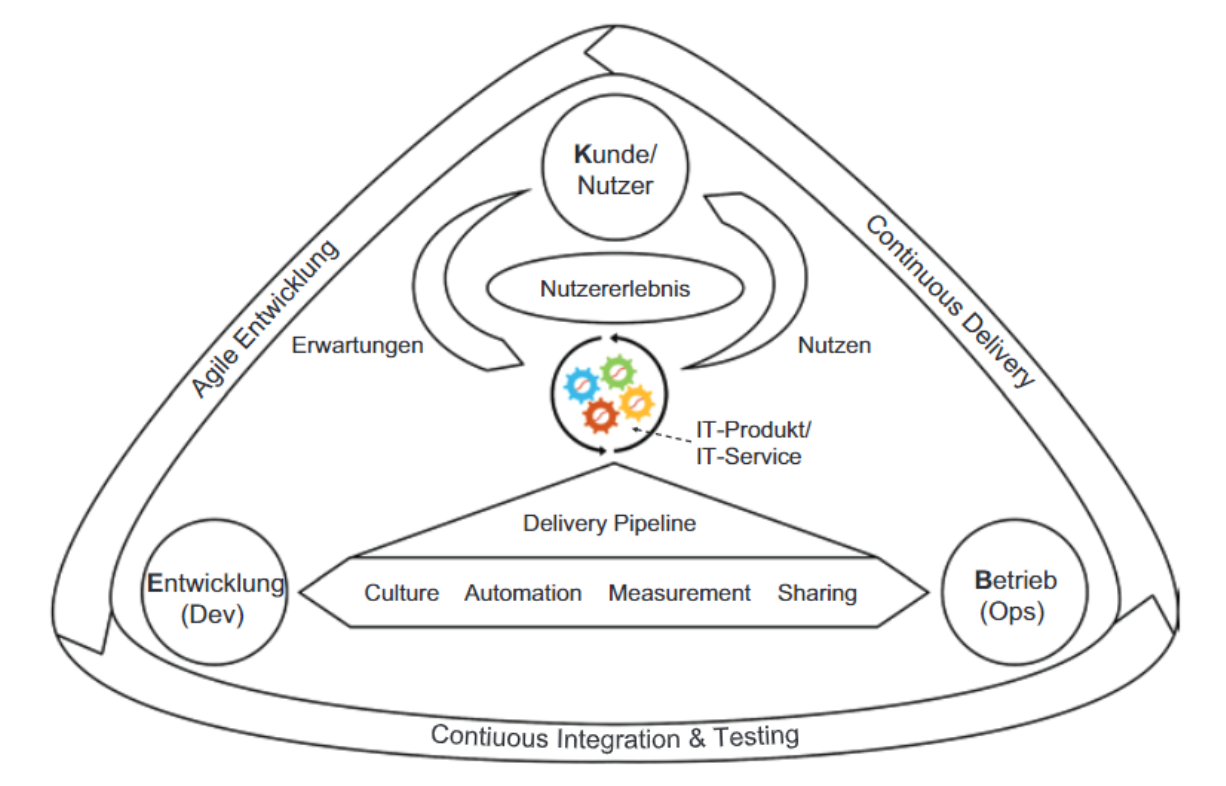
\includegraphics[width=1.0\textwidth]{gfx/devops_ueberblick.PNG}
 \caption{\citet{Alt2017}, S. 28, DevOps im Überblick\label{fig:devops}}
\end{figure}
\medskip
Abb. \ref{fig:devops} stellt das DevOps Lebenszyklus mit ihren jeweiligen kontinuierlichen Verfahren dar, die das Produkt und die Beteiligten umfassen. Agile Entwicklung, \ac{CI} und \ac{CD} sind jeweils Verfahren, die vor DevOps existierten \cite{Alt2017}. Sie werden in diesem Zusammenhang jedoch als ein kontinuierliches Modell gesehen, die eine Schnittstelle zwischen den Beteiligten herstellt und das Produkt dadurch am Leben erhält und wachsen lässt. Im Gegensatz dazu stehen sequenzielle Modelle wie \emph{Plan-Build-Run \cite{Koch2016}}, in der ein Prozess am Ende als abgeschlossen gilt. Das Wesentliche an diesem Modell (Abb. \ref{fig:devops}) ist ein Kontinuitätsprinzip \cite{Alt2017} der Prozesse auf allen Ebenen.

\paragraph{ITIL}
\citet{Alt2017} beschreiben ITIL im Rahmen des Innovationsdrucks vom IT-Management.
Viele Organisationen haben ihre Leistungen nach dem ITIL-Service-Lebenszyklus strukturiert und den Ablauf an den ITIL-Prozessen ausgerichtet. ITIL bedingt die Kombination von Zweckmäßigkeit \enquote{Utility} und Einsatzfähigkeit \enquote{Warranty} für einen Wertbeitrag eines Services auf das Geschäft. Zweckmäßigkeit wird durch die Realisierung einer geforderten Funktion oder durch die Beseitigung einer Einschränkung erreicht. Als Qualitätsmerkmal gilt die Einsatzfähigkeit. Sie bezieht sich auf eine ausreichende Verfügbarkeit, Kapazität, Kontinuität und Sicherheit. Es ist Notwendig das bisherige Verständnis von IT-Services um das Kriterium \enquote{Innovationsbeitrag} zu ergänzen. Services müssen sich in einer Innovationskultur bezüglich ihres Beitrags zur Innovationsgenerierung messen lassen.

\paragraph{Design Thinking}
Design Thinking gehört zu den kreativen und innovativen Prozessen für die Gestaltung von Lösungen. Ihr wesentlicher Merkmal ist die agile und zeitnahe Bereitstellung von Prototypen \cite{Alt2017}.

\paragraph{IT4IT}

\paragraph{Infrastructure as Code}
Eine wichtige Voraussetzung für DevOps ist die Automatisierung von Prozessen, die vor allem im Bereich von materiellen Ressourcen, wie Hardware bisher schwierig war. Das Prinzip der \emph{Dematerialisierung} ist auch ein wichtiger Bestandteil der digitalen Transformation.
\ac{IaC} ist die Abstraktion von IT-Infrastrukturen und -Ressourcen auf eine Ebene analog zu einer Programmiersprache. Diese Analogie impliziert schon eine Automatisierung in der Ausführung der jeweiligen Prozesse. Über Schnittstellen kann die Infrastruktur angefordert und konfiguriert werden. Die Bereitstellung von IT-Ressourcen kann aufgrund der steigenden Anforderungen an die IT-Architektur \cite{Brockhoff2006, Bussmann2006, Alt2017} nicht mehr manuell erfolgen und muss automatisiert werden. Daher ist dieser Ansatz für die Umsetzung von DevOps erforderlich.

Nach Alt et al. \cite{Alt2017} sorgt eine programmierbare Infrastruktur für Flexibilität, senkt die Fehlerrate und beschleunigt die Installation und Konfiguration von Systemen.

\paragraph{Infrastructure as a Service}
\ac{IaC} bietet eine Möglichkeit die Infrastruktur programmierbar zu gestalten und ihre Prozesse dementsprechend zu automatisieren. An ihre Schnittstellen anknüpfend entsteht die Möglichkeit eine Plattform für eine serviceorientierte IT-Architektur aufzubauen. Hieraus resultiert \ac{IaaS} als Delivery-Modell \cite{Alt2017} für die IT-Ressourcen. Während sich \ac{IaC} auf das Deployment von Infrastrukturen konzentriert, ist \ac{IaaS} die Delivery-Pipeline im Bereich der IT-Infrastruktur. Ihre Aufgabe ist analog zu \ac{CD} das Nutzererlebnis der Entwickler, die Entwicklung zu verbessern. Das Produkt ist in diesem Fall die Infrastruktur, die als ein Service bereitgestellt wird.

\paragraph{Cloud-Computing}
Ansätzen wie \ac{IaC} und \ac{IaaS} entstanden aus dem Bereich Cloud-Computing \cite{Alt2017}. Sie stellen mittlerweile eine Plattform für IT-Infrastruktur und ganze IT-Architekturen zur Verfügung und bieten eine Möglichkeit die Kosten des IT-Betriebs durch Auslagerung erheblich zu senken. Beispiele für Cloud-Plattformen sind \ac{GCP}, \ac{AWS} und Microsoft Azure.

Cloud-Plattformen sich darauf IT-Ressourcen dem Kunden nach Bedarf extern zur Verfügung zu stellen. Wenn der Bedarf sinkt, werden die Ressourcen an eine andere Stelle allokiert. Bezahlt wird hierbei die beanspruchte Zeit der Ressourcen. 


\paragraph{Software as a Service}

\paragraph{Platform as a Service}

\paragraph{Microservices}

\paragraph{Container-Virtualisierung}

\paragraph{Container-Orchestrierung}

\paragraph{Google Kubernetes Engine}

\begin{figure}[htbp]
 \centering
 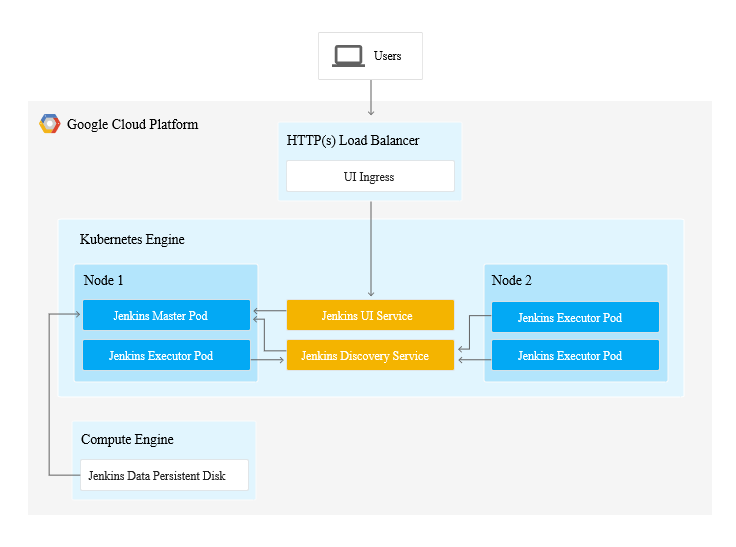
\includegraphics[width=1.0\textwidth]{gfx/jenkins-kubernetes-architecture.png}
 \caption{Deployment von Jenkins in einem Kubernetes Cluster mit mehreren Knoten \cite{Google:GKEJenkins}\label{fig:gkejenkins}}
\end{figure}

Google beschreibt in \cite{Google:GKEJenkins} einen Ansatz für eine skalierbare Architektur von Jenkins mit der \ac{GKE}.

In Abb. \ref{fig:gkejenkins} werden die Komponenten in mehreren Knoten, genannt Nodes zusammengefasst. In Node 1 befindet sich der Jenkins Master. Innerhalb dieses Nodes kann der Jenkins Master repliziert werden. Im gleichen Node oder in weiteren Nodes können die Jenkins Agenten, genannt Jenkins Executor, erzeugt werden.

Der Load Balancer aus der \ac{GKE} arbeitet vollautomatisch und erfordert nur wenige Parameter zur Konfiguration. Das reduziert den Aufwand in der Entwicklung dieser Architektur erheblich.

So lange in einem Node genug Ressourcen frei sind können weitere Container in so genannten Pods erzeugt werden. Zudem können beliebig viele weitere Nodes aktiviert oder erzeugt werden. Ein Node ist in \ac{GKE} eine virtuelle Maschine aus der Computing Engine.
\medskip
\\
Daraus resultiert eine hohe Flexibilität für die Skalierung der Anwendungen. Diese können sowohl vertikal anhand der Ressourcen von den Nodes, als auch Horizontal über die Aktivierung von weiteren Nodes oder Pods skaliert werden. Vor allem bestehen für die horizontale Skalierung mehrere Abstraktionsebenen.

\paragraph{Minikube}
%
%
%
%
\section{Ausgangssituation: CI in Banken}
\label{grundlagen:ci-in-banken}
\medskip
\\
In diesem Abschnitt wird die Ausgangssituation beschrieben, aus der die Problemstellung definiert wurde. Sie gibt einen kleinen Einblick wie die Rahmenbedingungen für Entwickler in der IT einer Bank mit modernen Methoden wie DevOps aussehen könnten und wo die Grenzen für Veränderungen liegen. Von diesem Standpunkt aus wird ein erster Lösungsweg vorgeschlagen gängigen Standards aus dem Stand der Technik. 

\paragraph{Softwareentwicklungsumgebung}
Die \ac{SEU} bezeichnet in dieser Arbeit ein zentrales Netzwerk für die eigene Softwareentwicklung in einer Bank. Unter anderem müssen in Banken Test-, Integrations- und Produktionsumgebungen getrennt werden \cite{MaRisk:2017}.
\medskip
\\
Die \ac{SEU} ist eine Umgebung innerhalb welcher die Integration von Quellcode aus dem \ac{SCM} durchgeführt und anschließend mithilfe einer Delivery Pipeline an die \ac{CD} Gruppe ausgeliefert wird. \ac{CD} hat anschließend die Aufgabe die Anwendung abzunehmen und in die Produktionsumgebung bereitzustellen.

Die Integrationsumgebung ist einer \ac{CI} Gruppe zugehörig. Ihre Aufgabe besteht in der Weiterentwicklung der Systeme und Anwendungen für die \ac{SEU}. Sie kann als eine Plattform für die unterschiedlichen Projektgruppen für Anwendungsentwicklung gesehen werden.
Die Zusammenarbeit der \ac{SEU} ist nach \emph{DevOps} Methoden ausgerichtet (Abb. \ref{fig:devops}), mit der Besonderheit, dass die Kunden von \ac{CI} die Entwickler aus den Projektgruppen sind. Die \ac{CI} Gruppe ist aus Sicht der Gesamtorganisation in Wahrheit ein kleiner Betrieb für die Entwicklung. Sie ist auf den tatsächlichen IT-Betrieb der Organisation bezüglich der Infrastruktur angewiesen. Wie bereits erwähnt sind die Umgebungen streng voneinander getrennt \cite{MaRisk:2017}, woraus die hohen Laufzeiten für die Bereitstellung von angeforderten \ac{VMs} stammen. 
\medskip
\\
Aus diesem Grund könnte die Verfügbarkeit der \ac{SEU} Systeme gefährdet werden. Der IT-Betrieb ist hierbei Service- aber auch Prozessorientiert. Daher könnte die Skalierbarkeit durch externe Infrastrukturen mit effizienteren Prozessen möglicherweise erreicht werden. Die Anbindung der \ac{SEU} an eine externe Cloud stellt eine wesentliche Veränderung und Auslagerung nach \cite{MaRisk:2017, BAIT:2018} dar. Eine Entscheidung für oder gegen eine externe Cloud ist daher eine strategische Entscheidung mit tiefgreifenden Auswirkungen, die analysiert werden müssen \cite{recht/Bornemann2018, MaRisk:2017, BAIT:2018}.
\medskip
\\
Die \ac{SEU} könnte jedoch innerhalb des eigenen Netzwerks über Container-Technologie flexibel und skalierbar implementiert werden. Die gängigen Lösungen \cite{Pathania2017, Google:GKEJenkins} unterliegen jedoch aufgrund diverser Besonderheiten der Legacy-IT in einigen Finanzinstituten \cite{Brockhoff2006, Bussmann2006} aufwändigen Anpassung, die gegebenenfalls die Effizienzsteigerung der neuen Technologie negieren könnte. Im kleinen Umfang könnten jedoch einzelne Komponenten modularisiert und mit Containern leichtgewichtig und skalierbar umgesetzt werden \cite{Bussmann2006}, (Par. 2 \ref{ansatz:modularisieren}.

\paragraph{Anwendungen für die Build-Pipeline}
\begin{itemize}
    \item \textbf{Gitlab}, als \ac{SCM}
    \item \textbf{Jenkins}, als \ac{CI} Plattform für die Build-/ Delivery-Pipeline
    \item \textbf{Artifactory}, als Repository für verwendete Artefakte
\end{itemize}


\paragraph{Nachvollziehbarkeit der SEU}
Die \ac{SEU} sollte ist aus mehreren Gründen möglichst nachvollziehbar zu gestaltet. Eine flexible Umgebung setzt auch Wartbarkeit und Anpassungsfähigkeit voraus. Dies ist durch die Verwendung von gängigen Standards möglich. Systeme sollten möglichst unabhängig von einzelnen Verantwortlichen verständlich und offen sein. Eine Individualisierung von Systemen sollte möglichst vermieden werden. Sie sollten auf einen gemeinsamen Nenner gebracht werden.

Dadurch kann eine schnelle Anpassung der Systeme an neue Technologien und Methoden erfolgen. Gleichzeitig können Systeme für neue Geschäftsmodelle in kurzer Zeit weiterentwickelt werden. Während einer Störung der Systeme oder in Krisensituationen kann auch schnell reagiert werden.

Dies hat auch einen positiven Effekt auf interne Kontrollverfahren. Die Umgebung ist nicht nur verständlicher für den Prüfer sondern auch sicherer durch die Verwendung von bereits geprüften Standards.

Nachvollziehbarkeit wird in Banken auch für die Rückverfolgung von Softwareartefakten vorausgesetzt. In der Praxis müssen Ergebnisse aus der Entwicklung rückverfolgbar sein bis auf den Quellcode, der Anforderung und dem Prozess aus der sie entstanden sind.

\paragraph{Repository für Artefakte}
Eine Standardsoftware hierfür die Anwendung Artifactory. Diese speichert in einem Snapshot die Ergebnisartefakte aus dem Build-Job und die zum erstellen verwendeten Artefakte. Das Artifactory wird ebenfalls verwendet, um Tools und Libraries für den Build zu beziehen. Dazu wird Artifactory entweder als Proxy für den Zugriff auf ausgesuchte öffentliche Repositories verwendet oder die Ressourcen werden in der Artifactory Instanz hinterlegt.

\paragraph{DevOps mit Mircroservices}
Daraus folgt, dass einzelne umfangreiche Systeme für die \ac{SEU} keine Flexibilität bieten. Für automatisierte Prozesse und skalierbare, flexible Umgebungen können die Anwendungen aus der \ac{SEU} in noch kleinere Module aufgeteilt werden. Insbesondere ist es wichtig, dass einzelne Komponenten der Integrationsplattform trennbar sind und unabhängig voneinander laufen. Komponenten sollten \enquote{self-contained} aufgebaut werden. In folge dessen sind sie flexibler können auch unabhängig voneinander skaliert werden. Das würde Engpässe erheblich reduzieren. Die Eliminierung von Abhängigkeiten sorgt für eine bessere Nachvollziehbarkeit, da hierbei gängige Standards angewendet werden können.

\paragraph{Skalierung von Jenkins mit Kubernetes}
\label{jenkins:skalierung}
Üblicherweise werden Anwendungen in Kubernetes mit Replikas skaliert. Das heißt in der Praxis, dass eine neue Instanz der Anwendung erzeugt wird und ein Load-Balancer die Anfragen unter den verschiedenen Instanzen verteilt. Das resultiert in der vorwiegend horizontalen Skalierung von Anwendungen. 

Jenkins besteht bei einer Konfiguration mit verteilten Builds aus mehreren Komponenten. Ein Jenkins Master, welche die Anfragen bearbeitet und Build-Jobs triggert und ausführende Agenten für die Verteilung von Builds. Die Komponenten sollten getrennt voneinander skaliert werden, da sie vorwiegend für die ausführenden Komponenten erforderlich ist. 

Hierfür gibt es in Kubernetes mehrere Abstraktionsebenen. Die größte Einheit, die die ganze Architektur zusammenfasst ist der Cluster. Dieser besteht aus mehreren Knoten, die jeweils mehrere Pods beinhalten. Die Knoten sind virtuelle Maschinen und enthalten die Hardware. Innerhalb dieser Knoten werden die Container ausgeführt. Diese sind noch einmal unter Pods zusammengefasst, die eine Arbeitseinheit oder Service darstellen. 
\medskip
\\
Ein sinnvoller Ansatz ist die ganze Anwendung innerhalb eines Knotens aufzubauen und sie durch Replikas der Knoten zu skalieren. Dabei sollte die Anwendung modularisiert werden und in unabhängig voneinander skalierbare Microservices aufgeteilt werden. Anwendungen können komplex sein und ein Engpass entsteht in wenigen Bereichen, sodass nicht die ganze Anwendung repliziert werden muss. In der Praxis werden die Funktionen der Anwendung in mehreren Containern aufgeteilt, die miteinander kommunizieren. Die Replikation von Containern bewirkt, dass Anwendungen nur in den Komponenten skaliert werden, in der es erforderlich ist. Diese Praxis schafft Redundanzen ab und und sorgt für einen Wirkungsgrad in der Nutzung von IT-Ressourcen.

\paragraph{Anlegen eines Kubernetes Clusters für Jenkins}
Pathania beschreibt in \cite{Pathania2017}, wie Jenkins mit \ac{GCP} und Kubernetes und Docker skaliert werden kann. Hierbei geht er genau auf die technische Konfiguration von Kubernetes und der \ac{GCP} ein.